\chapter{数学导论 - 概述}

\begin{figure}[ht]
  \centering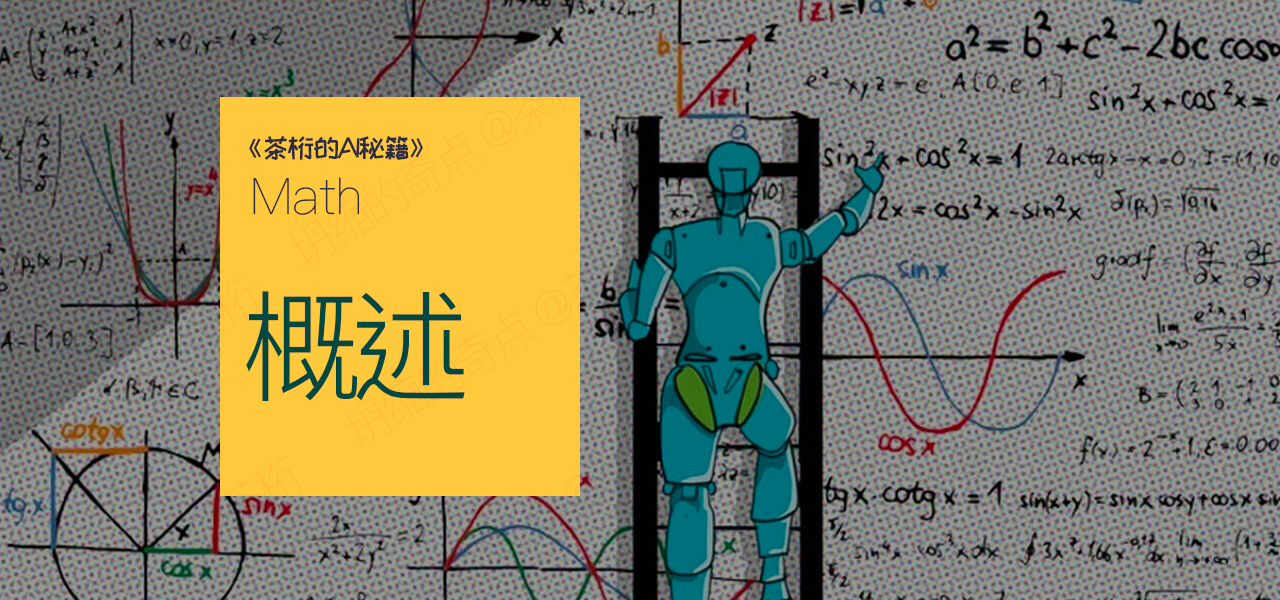
\includegraphics[width=1\textwidth]{asset/茶桁的AI秘籍_Math_1.png}
\end{figure}

\newpage
\begin{quotation}
  因为PDF展示动图不方便, 当本电子书涉及到gif动图的时候, 并未直接展示而是给到了连接, 还望见谅. 
\end{quotation}

\section{前言}

大家好, 我是茶桁. 

在之前的一个多月前, 我有了写一个AI系列的想法, 起名为《茶桁的AI秘籍》, 简单规划之后, 于7月27日发出预告, 然后历时二十多天将近一个月\footnote{按本文完成时间而非电子书时间, 具体可以前往公众号「坍缩的奇点」查看. }, 完成了其中《Python篇》的写作.  

不知道其中的内容对大家是否有帮助呢?

那么今天我又回来了, 根据规划, Python以及相关第三方科学计算库只是我们基础工作的一小部分, 而很大一部分基础工作都还未进行. 

那么这次, 我依然给大家带来的是基础部分, 让我们进入 \href{https://mp.weixin.qq.com/mp/appmsgalbum?__biz=MzA4NzE4MDQzMg==&action=getalbum&album_id=3074770001140400130&from_itemidx=1&from_msgid=2648748768#wechat_redirect}{《茶桁的AI秘籍 - 数学篇》}. 

本节课的内容是「数学篇」的第一节课. 本节是一个导论. 我会为大家介绍一下这门课一些理论, 还有微积分、线性代数、概率统计里面一些比较基础, 和AI结合非常紧密的一部分, 难度并不会很大. 

觉得自己数学能力还不错的, 第一节课可以不用看, 直接去看后面的课程. 第一节课, 我们放松一点. 这节课难度真的不会特别的大, 主要是带大家了解一些比较有趣味性以及AI方面一些基础性的数学知识. 

数学对于计算机编程来说重要性是毋庸置疑的, 更何况我们现在不仅仅是编程, 而是走在「人工智能」的路上. 可以说, 数学应该是最重要的基础. 那从本节课开始, 就让我们进入「人工智能的数学基础课」. 

我们在学习AI的过程当中可能会遇到的一些关于数学方面的一些东西, 比如说线性代数里面的这个矩阵运算, 比如说这个求导, 还有一些概率统计, 图论方面的一些东西. 

如果您觉得自己对于微积分, 线性代数, 概率统计这些内容自认为掌握的还不错的同学, 其实是可以不用看了. 如果大家是从文科转过来或者说以前上的数学很多年了也忘的差不多了, 那可以来听听这些课. 

本节课的内容是「数学篇」的第一节课. 本节是一个导论. 我会为大家介绍一下这门课一些理论, 还有微积分、线性代数、概率统计里面一些比较基础、和AI结合非常紧密的一部分, 难度并不会很大. 觉得自己数学能力还是不错的, 这第一节课呢可以不用看, 可以直接去看后面的课程. 第一节课, 我们放松一点. 这节课难度真的不会特别的大, 主要是带大家了解一些比较有趣味性以及AI方面一些基础性的数学知识. 

首先我们会说一下为什么需要数学、人类从历史到现在是怎么表示数字的、计算机是怎么样对数字进行处理的, 还有我们也会说到计算机其实并不是像我们想象的那样无所不能, 它其实也有很多的漏洞. 然后接下来这几个模块我们就会分别去介绍微积分的基础, 主要是导数以及矩阵, 还有随机变量、图论里面这个图的概念. 

\section{为什么需要数学}

这个问题在古代有一个很明确的答案, 就是不管你是要丈量土地, 还是说要建立这种大型的水利工程, 或者说其他的工程项目, 你都不可避免的需要做很精确的这种数学计算. 

比如说古代皇宫他的新建, 或者说帝王这个陵墓的新建, 他都是需要一些非常精确的这种计算的, 包括从风水的角度. 而且大家都知道, 我们国家天文立法的水平其实是非常高的, 这也来源于我们在古代就建立起一套非常严密的数学体系. 

还有一个和生活比较贴切的例子就是算盘. 算盘不光是帐房先生用, 其实在古代用的面非常广, 我们知道就是现在有一门速算的这种能力叫做「珠心算」, 珠心算其实就是通过让学员在这个珠算上面去进行大量的训练. 训练到他们可以在自己的心里面去模拟出这么一个算盘出来, 然后他们就可以在心里面打这副算盘, 达到珠算的一个速度. 

\begin{figure}[ht]
  \centering
  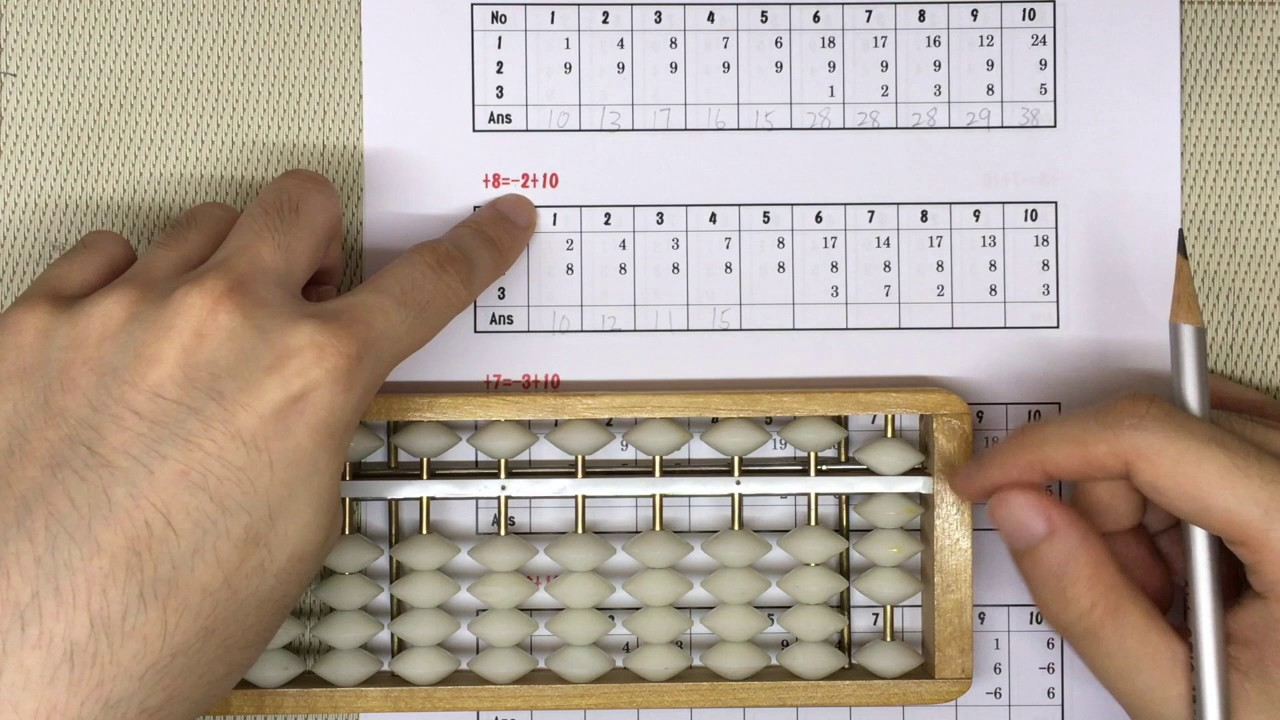
\includegraphics[width=0.5\textwidth]{asset/1c84c0f7-5335-4252-88ac-5e08192d89c3.png}
  \caption{}
  \label{fig:img2_1}
\end{figure}

那现代为什么我们需要数学呢?

大家可能会想到的就是因为高考得考对吧?大家都得拿着这个敲门砖去考大学, 然后将来进入社会. 

这个确实是一个, 不光是我们这门AI课程所需要涉及到, 在其他的一些科技领域, 比如说芯片制造、航空工程, 包括化工其实都是需要大量的数学. 

同样的, 在我们的商业活动当中也是可以见到数学的影子. 比如说大家知道量化金融分析、量化交易, 这个也是需要数学的, 需要大量数学计算. 而有一点大家可能想不到, 就是政治学其实也是需要数学的. 在西方的政治学其实是作为一个类似于自然科学的东西被研究的, 它那上面有非常详细的政治选举策略之类的内容, 甚至还融合了博弈论这些东西. 

\begin{figure}[ht]
  \centering
  
\includegraphics[width=0.5\textwidth]{asset/7e4f1c0f-936f-4b29-82e1-5294232218f3.png}
  \caption{}
  \label{fig:img2_2}
\end{figure}

\section{人类如何表示数字}

我们来说一下史前文明时期人类是怎么表示数字的. 

其实在地球的不同地区, 不管是在中国还是在外国都非常不约而同的出现\textbf{结绳记事}的方法. 

(图:\ref{fig:img2_3})是中美洲的一个印加文明, 它用来表示数字以及一些事物的. 这个方法就是在这个绳子上面打结. 

\begin{figure}[ht]
  \centering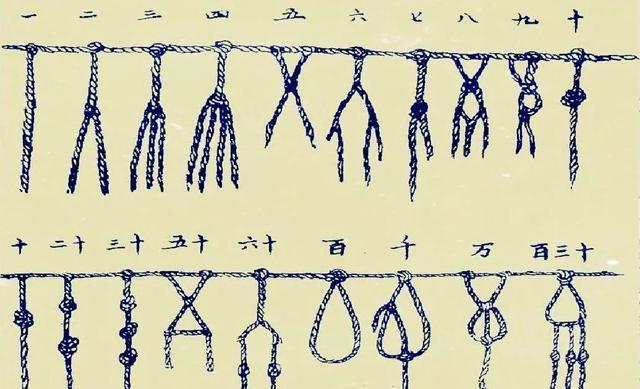
\includegraphics[width=0.5\textwidth]{asset/73a095be-4ca9-4065-abb0-5d919706b1dd.png}
  \caption{}
  \label{fig:img2_3}
\end{figure}

非常惊奇的是咱们中国古代也有类似的这种体系(图:\ref{fig:img2_4}). 

\begin{figure}[ht]
  \centering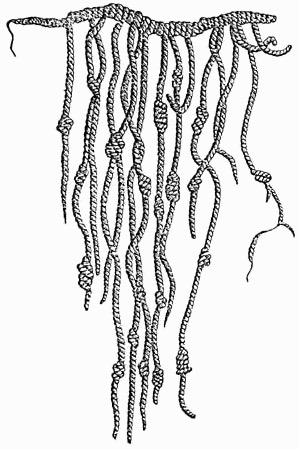
\includegraphics[width=0.4\textwidth]{asset/840839db-800f-44f2-8f4a-b7e17b896222.png}
  \caption{}
  \label{fig:img2_4}
\end{figure}

我们可以看到这上面不同的结对应的不同的数字. 这就是古人的一种基数体系. 然后等到文明在进一步发展了之后, 我们可以看到四大文明古国都发出了自己各自的文字符号体系. 

图:\ref{fig:img2_5}是古巴比伦人的楔形文字. 为什么叫楔形文字?这个楔在汉语里面的意思呢就是钉子. 为什么这种文字是这种楔形的呢?是因为它们是把这个竹片或者刀片在这种还没有干的泥板上面去刻字, 而刻出来的就是这种坑洼的形状. 

\begin{figure}[ht]
  \centering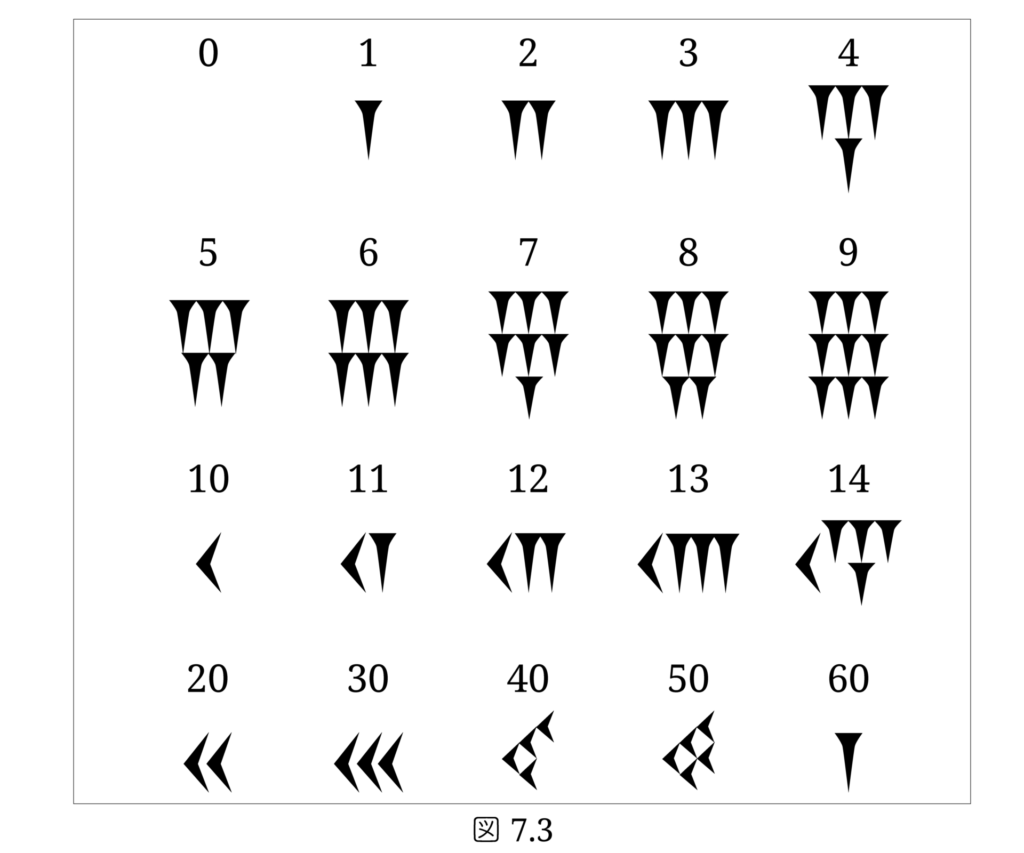
\includegraphics[width=0.5\textwidth]{asset/df03e920-b04e-493d-aab6-b5ffb16eb0bf.png}
  \caption{}
  \label{fig:img2_5}
\end{figure}

图 \ref{fig:img2_6} 是古埃及人的象形文字. 他们这个数字体系非常有特色, 融合了宗教的因素在里面. 比如说这个1,000, 他是用一个睡莲的图案来表示, 手指呢代表了1万, 青蛙代表了10万, 天神呢代表了100万. 

\begin{figure}[ht]
  \centering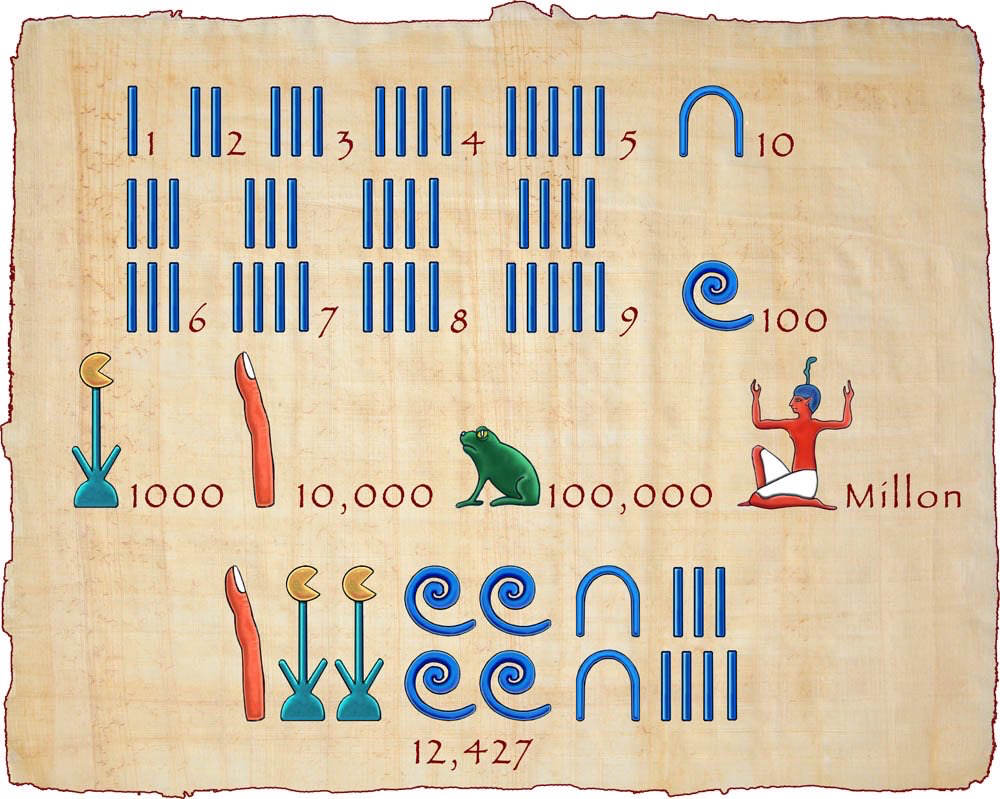
\includegraphics[width=0.5\textwidth]{asset/191cd6bc-63e3-4090-af11-bf3e7de6f4db.png}
  \caption{}
  \label{fig:img2_6}
\end{figure}

接着就是我们国家的(图:\ref{fig:img2_7}). 中国在甲骨文时代的文字技术体系还是有很明显的这种象形文字影子在里面, 尤其是像这个1万、3万, 在我们看来可能现在像蝎子一样. 

\begin{figure}[ht]
  \centering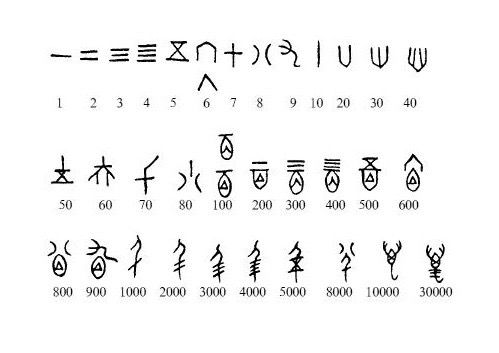
\includegraphics[width=0.6\textwidth]{asset/56174953-293d-47aa-893c-52ab80acacd9.png}
  \caption{}
  \label{fig:img2_7}
\end{figure}

然后就是古印度的数字体系(图: \ref{fig:img2_8}). 古印度有一点比较特殊. 我们知道其实阿拉伯数字不是阿拉伯人发明的, 这一点可能大家都知道, 这个是古印度人发明的, 只不过是由阿拉伯商人传到了欧洲, 所以欧洲人就把它称为阿拉伯数字. 虽然和我们现在使用的阿拉伯数字不太一样, 但是他有一些非常重要的概念已经被提出了. 比如说古印度人已经有这个0的概念了, 而且他有这个进位的概念. 什么叫进位呢?你看, 我们在其他的文明这个字符体系里面, 比如说这个10, 它是用一个特别的符号来表示的, 但是在古印度的数字符号体系里面是用了一个一和一个0, 这个0占一位来表示这个10. 这点在我们现代人看来其实好像没有什么可说的, 大家可能会觉得不应该就是这样吗. 但其实这个在古代是一个非常了不起的一个成就. 

\begin{figure}[ht]
  \centering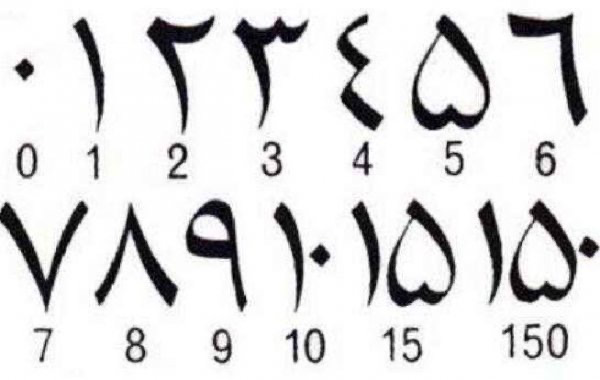
\includegraphics[width=0.4\textwidth]{asset/02cf4930-6fd5-40ab-b755-155d4bcf1fa1.png}
  \caption{}
  \label{fig:img2_8}
\end{figure}

同样的有一个文明需要说一下, 就是古玛雅文明. 古玛雅文明为什么放在这里说, 是因为他也提出了零和进位的这种概念. 他这个数字体系有两种, 一种呢是那种点横线的体系, 还有一种呢是和宗教息息相关的用神之的头像去表示数字的这种体系. 而他这个零和进位概念的提出比印度人和其他的古文明甚至还要早了将近一两千年. 所以这一点是非常了不起的, 很多这个科学家还有考古学家都觉得这个玛雅文明是一个外星文明的后代, 不然他不可能在其他四大文明古国之前一两千年就有了零和进位的这个概念. 

\begin{figure}[ht]
  \centering
  \begin{minipage}[t]{0.4\textwidth}
    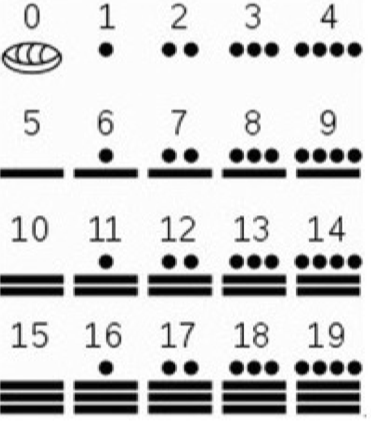
\includegraphics[width=\textwidth]{asset/265551e1-4fa0-4611-b795-3835b8967cf0.png}
    \caption{}
    \label{fig:img2_9}
  \end{minipage}%
  \hspace{1em}
  \begin{minipage}[t]{0.4\textwidth}
    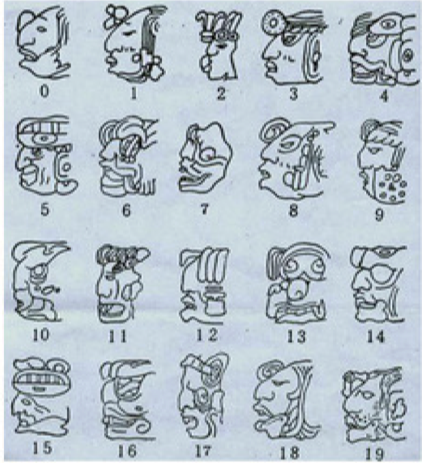
\includegraphics[width=\textwidth]{asset/71bac7f0-1042-47b2-a771-34b5eb04b656.png}
    \caption{}
    \label{fig:img2_10}
  \end{minipage}
\end{figure}

零我们会经常遇到它, 但是它不光是表示没有, 还表示着占位. 就比如说在进位里面它这个0如果在个位就表示占着个位, 然后如果这里再来个 1 它就表示0前面的 1 表示10, 这是一个非常重要的概念. 

\section{计算机可以做什么?}

\begin{figure}[ht]
  \centering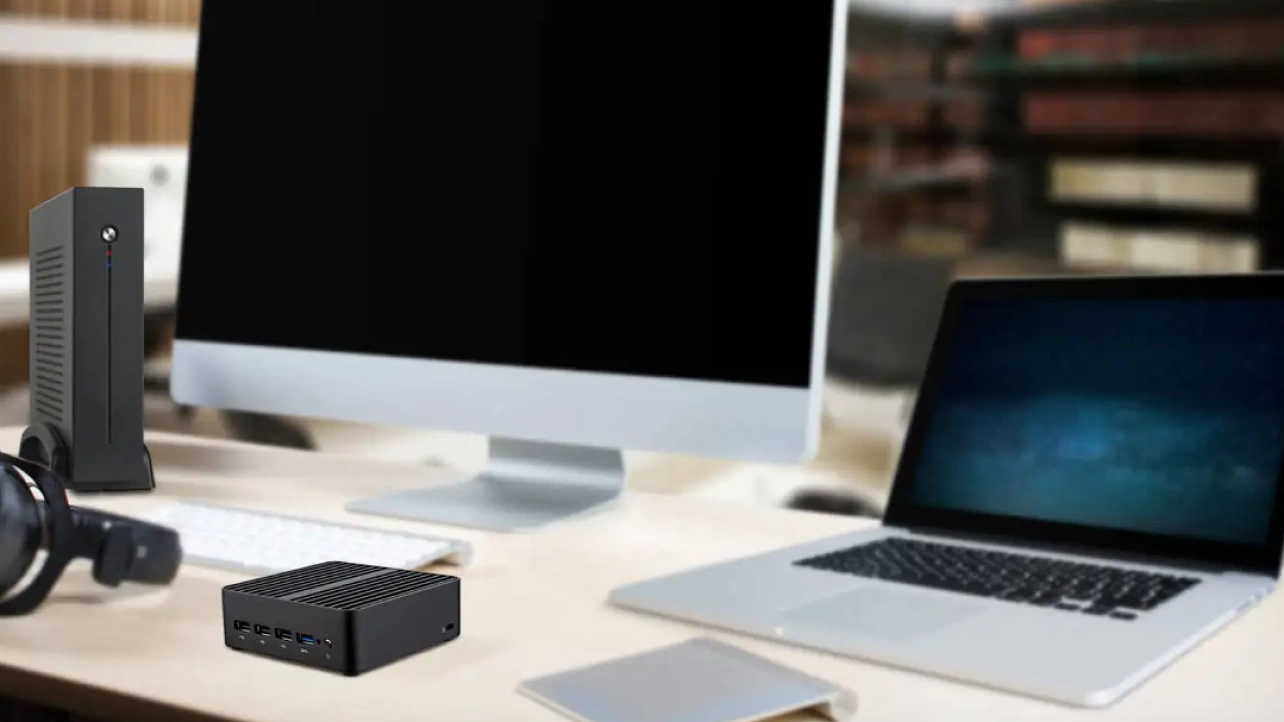
\includegraphics[width=0.8\textwidth]{asset/7b8b9bd7-b7db-4420-bcce-537d0be46a31.png}
  \caption{}
  \label{fig:img2_11}
\end{figure}

这个用途就太多了对吧, 像这个烟花一样, 散发到空中然后太多太多了. 

比如说我们可以用计算机去做图像处理. 说简单一点话就是PS或者说美颜, 我们可以对这个音频信号进行一个处理, 大家用这个百度啊或者高德导航啊能听到各种名人的这个声音, 其实那个真的是让名人说那么多的话吗》不是的, 其实可能也就是让那些人说个一两句两三句然后就根据他们这个声信号去合成, 用他们的发音特征, 而说出来这种这种语音. 很神奇对不对?

然后还有比较常见的:word、PPT、Excel这种字处理软件都是用计算机可以去做的. 包括我们有一些做科研的同学应该很清楚, 很多科学建模这种模拟也是用计算机去做的. 很多东西我们没办法在现有的实验室条件下去做, 或者经费太贵了导师给不起, 所以这个我们也用计算机去做. 当然还有大家最感兴趣的就是游戏. 

那计算机他是怎么样做到的呢?

其实, 不管你是哪一种类型的数据:不管是图像也好、音频信号也好、还是处理文字、还是说科学计算游戏等等, 其实在计算机看来呢都是一样的. 在计算机看来呢它都是$0101$这种字符, 都是数据流. 在计算机看来是分不清什么是游戏、什么是图像、什么是音频. 不管哪一种类型的数据它都是$0101$这种数据流. 

那计算机如何去处理这个$0101$就很重要了. 

首先我们先来了解一下:这个$01$它是怎么样去做运算的. 

其实$01$二进制的运算和我们这个十进制的加减乘除没有什么区别, 可能最大的区别就是十进制它有$0123456789$这十个数字
来表示所有的数字, 而在二进制里面它只有$0$和$1$两个字符来表示所有的数字. 二进制里面$1+1$不是说等于2了, 它就是是$10$(不是十, 是一零), 2只是在十进制里面. \ref{tab:table2_1}

\begin{table}[ht]
  \centering
  \begin{tabular}{ll}
    \toprule
    二进制加减法则  & 二进制乘除法则 \\
    \midrule
    $0+0=0$ & $0 \times 0=0$ \\
    $1+0=1$ & $1 \times  0=0$  \\
    $0+1=1$ & $0 \times  1=0$  \\
    $1+1=10$  & $1 \times  1=1$  \\
    $0-0=0$ & $0 \div 1=0 $ \\
    $1-0=1$ & $1 \div 1=1$  \\
    $1-1=0$ & \\
    $10 - 1=1$ &  \\
    \bottomrule
  \end{tabular}
  \caption{ 二进制运算法则}
  \label{tab:table2_1}
\end{table}

接下来我来给大家说一下二进制和十进制的转换. 其实也很简单, 有小学基础就可以, 主要我们要搞清楚这二进制的数字它是表示着什么东西. 

我们知道对于一个十进制数而言它的百位上面数字, 比如我说一个数字345, 那它百位上面数字3就代表它有3个100, 十位上的4就代表4个十, 个位上的5就表示5个一, 所以十进制数的345是怎么样去计算的?他就是3乘以100再加上4乘以10再加上5乘以1, 结果就是十进制里面的345. 

同样的对二进制而言也是一样, 只不过二进制的底不一样, 它不是十进制里面的10. 咱们就把十进制里面这个10或者100给它换成2的零次方, 2的一次方, 2的二次方就行了. 

\begin{figure}[ht]
  \centering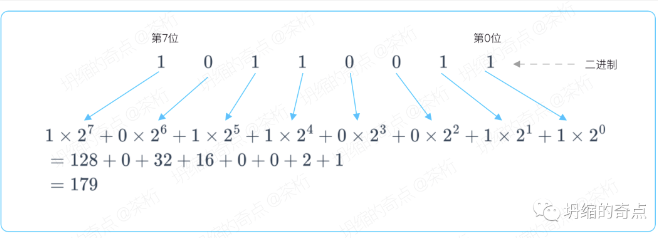
\includegraphics[width=0.8\textwidth]{asset/20231227140607.png}
  \caption{}
  \label{fig:img2_12}
\end{figure}

比如说图 \ref{fig:img2_12} 最右边一位就是二进制的个位数, 二进制的个位数它就代表了2的0次方. 其实我们想一下很容易理解, 我们刚才说到345里面这个5是5乘以1得来的, 那这个 1 是怎么得来呢?1 其实是10的0次方. 就是说这个是任何数除了0之外0次方都等于1. 二进制的十位数是2的一次方, 依此类推次数都会一直递增, 递增之后我们把前面的数值和这一位代表的位数相乘在一起. 把它所有结果相加就是十进制的数. 也就是:

\[
  1\times2^7+0\times2^6+1\times2^5+1\times2^4+0\times2^3+0\times2^2+1\times2^1+1\times2^0=179
\]

反过来,十进制的数怎么转成二进制呢? 这个你可以把它理解为不断除2取余法. 我们把这个数不断的去除以2, 与此同时得到余数, 一直这样除下去到什么时候为止呢?一直到被除数的商等于0. 现在我们得到了一连串的余数, 从下往上的顺序把它排列成这个二进之数, 如图 \ref{fig:img2_13}, 也就是$11010111$这个二进制数. 

\begin{figure}[ht]
  \centering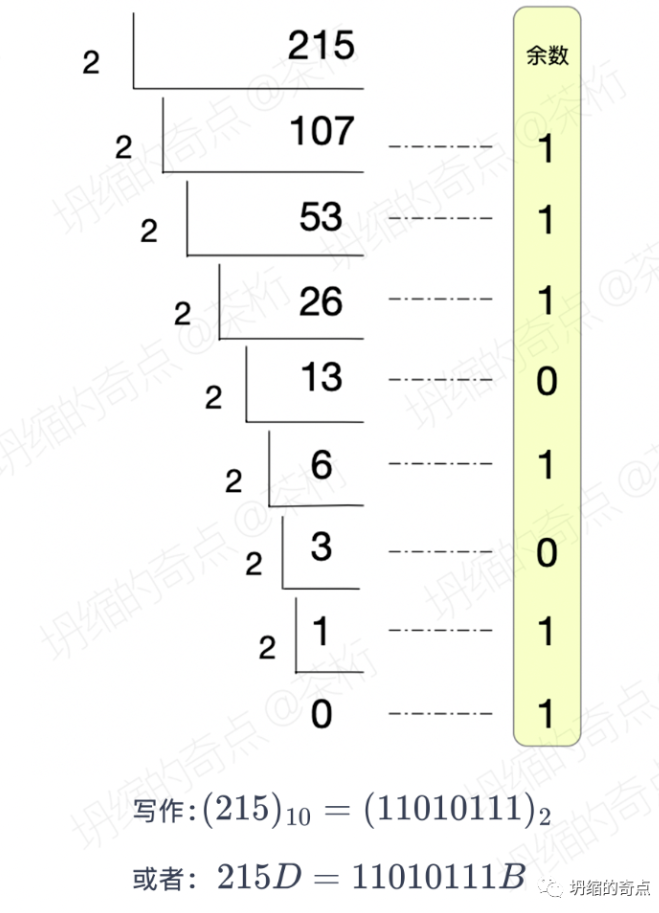
\includegraphics[width=0.4\textwidth]{asset/20231227140715.png}
  \caption{}
  \label{fig:img2_13}
\end{figure}

在第二种表示法中, D就是Decimer, 十进制的意思, B是Binary, 二进制的意思. 不难吧?

我们再说看看, 计算机是如何处理二进制数据的. 

之前我们讲过, 计算机无法处理十进制数, 所有的数据进入计算机都必须转成二进制的数据流. 那么大家是否会有疑问, 就是 $0101$ 这种数字, 计算机是怎么处理复杂的东西, 比如说游戏什么的. 

我来给大家看一张逻辑电路图(\ref{fig:img2_14}):

\begin{figure}[ht]
  \centering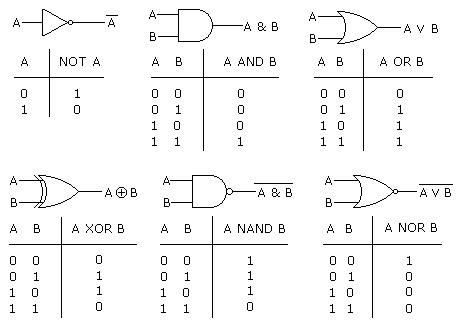
\includegraphics[width=0.5\textwidth]{asset/975a7883-49a7-4b15-8102-0352aebc5568.png}
  \caption{}
  \label{fig:img2_14}
\end{figure}

最上面的三个, 就是所有计算机电路机构的基础, 不管再怎么复杂的电路或者芯片, 最终都是以这三个为基础构建出来的. 

第一个叫做非门, 简单理解就是这个门是一个对着干的门. 你给我一个1, 我就给你个0, 你给我个0, 我就给你个1. 
第二个叫与门, 这个也好理解, 就是两个条件都必须满足才行, 就是你必须语文150分, 数学也150分, 爸爸妈妈才会给你买最新的iPhone 15 Pro. 那么这个门里, 我必须是两个条件都是1, 最后才会输出1, 否则都会输出0.
第三个叫或门, 从字面上看都很好理解了是吧?就是你语文「或者」数学考150分了都可以, 都会带你去吃一顿大餐. 那么这个门, 我们只要传入一个1就可以了, 就会输出1. 当然, 两个都是1的情况就是你两个都考了150分的情况, 当然更好对吧, 也会输出1, 也就是会出去吃一顿大餐. 

不管再怎么复杂的电路再怎么精密复杂的计算机, 其实都是由这种简单的小部件不断的累积不断的重叠加在一起获得的. 

那么下面三个我们这里就不解释了, 也不是重点. 对计算机原理感兴趣的同学可以去看看下面这节课:

计算机也并非无所不能. 我们都遇到过计算机突然崩溃不行的时候, 俗称蓝屏或者四国对吧?又或者, 计算机遇到了黑客, 或者我们不小心电脑中毒了, 致使个人信息全部被窃取了. 那这个都是计算机漏洞导致的. 

再比如说我们程序员经常遇到的, 就是我们写了一个程序:$0.1+0.2$, 我们会认为应该运行结果就是$0.3$对吧?但是实际上的情况呢?我们来做个实验看看:

\begin{figure}[ht]
  \centering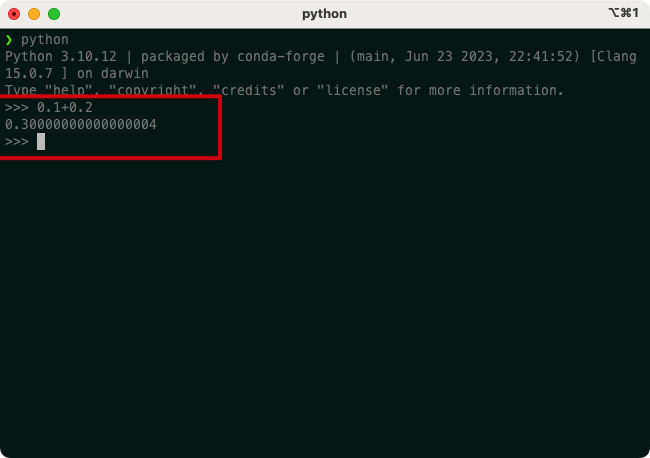
\includegraphics[width=0.6\textwidth]{asset/ef878802-961f-4168-9900-da12253d4b48.png}
  \caption{}
  \label{fig:img2_15}
\end{figure}

结果并没有如预期一样, 而是得到了一个意外的数字, 一大串的0后面跟了一个4.

我们需要从二进制的原理去理解, 之前我们学到的内容是十进制的整数转二进制, 用的是除2取余法, 但是小数的十进制转二进制, 需要用的方法不太一样, 叫做乘2取整法. 如图 \ref{fig:img2_16}:

\begin{figure}[ht]
  \centering
  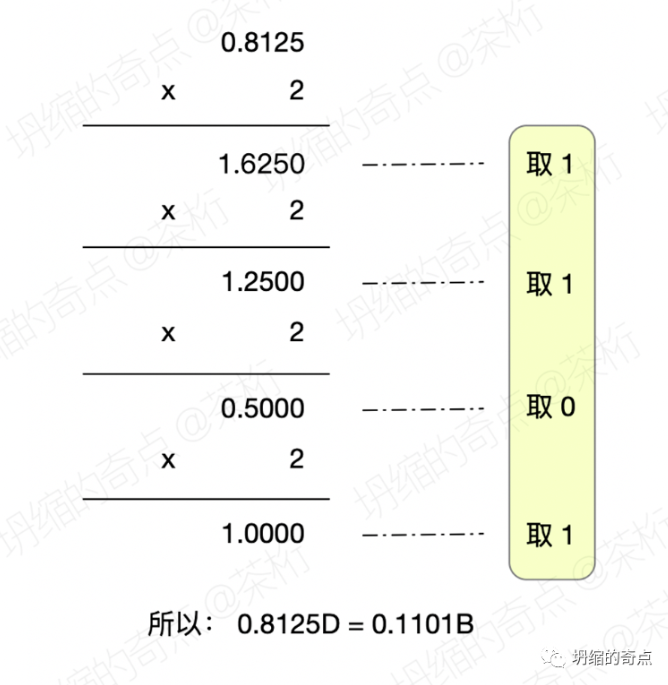
\includegraphics[width=0.4\textwidth]{asset/20231227140841.png}
  \caption{}
  \label{fig:img2_16}
\end{figure}

注意和整数的排序不同, 小数点后面的计算是从上往下顺序排列的. 

那二进制可以准确表示 0.1 吗? 我们按照刚才学的内容来算的话 就应该是 

\[0.000110011001100110011001100 ... \]

会无限循环下去. 

但是计算机内表示数字不可能无限循环下去, 是有限制的. 我们接着往下看:

\begin{figure}[ht]
  \centering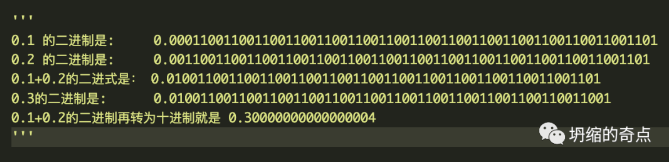
\includegraphics[width=0.8\textwidth]{asset/20231227140947.png}
  \caption{}
  \label{fig:img2_17}
\end{figure}

那为什么是这个位数呢?因为再循环下去也没有意义, 所以到保留到那一位之后就不往下取了. 我们也不用去数这些0和1到底是多少位, 知道是怎么回事就行. 我们看到第三行和第四行的表示并不一样, 这就是为什么我们计算$0.1+0.2$的时候并不会是$0.3$, 而是还跟着一串0接一个4. 

那这个问题我们怎么解决呢?因为很多场所下我们都需要高精度的数字. 其实也很简单, 转成整数再计算就行了, 因为整数转二进制没有这种问题, 比如说$0.1+0.2$, 我们计算$1+2$, 然后再除以10就可以了. 

在一些要求不是很高的应用场景内, 我们可以提高可表达数的精确度就能满足需求. 比如\textit{big decimer},  在Java这些语言里面都有. 

然后我们再来思考一下, 这种问题是二进制里才有的吗?其实并不是, 比如我们十进制就经常有无限循环小数对吧?比如说 $\frac{1}{3}$,  如果写成小数的形式也是一样, 3会无限循环下去. 所以这并不是二进制独有的问题, 所有的进制都会有这样的问题. 那么问题来了, $0.9999 ... $无限循环下去, 是否等于 1 呢?

其实答案为「相等」. 怎么证明呢?

我们说$1/3 = 0.333333 ... $,  那么$0.3333 ...  \times 3 = 0.9999 ... $,  等式右边乘以3了, 那左边也一样会乘以3,  得到$1/3 \times 3 =1$. 所以最后我们可以得出结论, $0.9999 ... =1$对吧?

然后我们来看, 人工智能是如何运转的?

人工智能是利用计算机这种强大的算力, 按照AI模型的规则实现特定的逻辑推断任务. 简单点说就是以前人能进行的思考、逻辑推理推断的活动我们现在希望计算机也可以有. 

有的同学可能会问:那计算机现在没有吗?计算机其实是一种自动化的程序, 这种规则的制定都是按照我们事前已经约定好的规则. 它只能按照我们既定的规则去做, 超出了这个规则之外是没办法去做的. 比如说我这个程序只会负责把林志玲的声音合成然后输出, 那我想让它生成郭德纲的就不行. 超出了能力范围, 它也不知道怎么去弄. 

人工智能就是希望他能让计算机拥有自我的思维逻辑推理能力, 不管是哪一种AI模型, 无论是现在特别火的大语言模型, 机器学习里面的深度学习、神经网络、还是说什么朴素贝叶斯都是
高度依存于我们现有的这种数学体系. 所以, 人工智能和数学息息相关. 

不过大可放心, 难度没有太大. 不会像数学系那样, 还让你去求什么「一致连续」、「区间套定理」、「7个定理循环证明」等等. 不可能是那样子的, 我们更多的是拿来用就行, 难度也不会特别的大. 

学习人工智能我们需要哪几个方面的知识呢?

主要是四个:1. 微积分;2. 线性代数; 3. 概率 \& 统计;4. 图论. 

相对来说, 前三个应用的会稍微偏多一点. 图论也会有一些应用, 比如说在一些图优化里面
或者网络搜寻会用到. 这四个内容我们都会接触到. 

好了, 之前铺垫了那么多. 那接下来就正式开启了数学基础的模式. 